\documentclass{article}
\usepackage[margin=1in]{geometry}
\usepackage{siunitx}
\usepackage{array}
\usepackage{booktabs}
\usepackage{hyperref}
\usepackage{graphicx}

\begin{document}
\author{Sachith Dunatunga}
\title{16.930 PS2}
\maketitle

\section{Area and Perimeter of a Circle}
As before, the code to generate everything is available online at github at \url{https://github.com/neocpp89/16.930-ps2}.

The tables \ref{tbl:area1}, \ref{tbl:area2}, and \ref{tbl:perimeter} look mostly as expected, but the cubic seems to be off.
Looking at the difference tables in tables \ref{tbl:diffarea1}, \ref{tbl:diffarea2}, and \ref{tbl:diffperimeter} we see that there is indeed something strange.
I believe the calculation of the jacobian or normal must be done incorrectly, but my simple, lower order tests were not able to see the problem.

\begin{table}
\caption{Here we show the results for the volume integral over the circular mesh.}
\centering\begin{tabular}{c | c c c}

Order & size = 0.4 & size = 0.2 & size = 0.1 \\
p = 1 & 2.99998005 & 3.120035198 & 3.135911097 \\
p = 2 & 3.141104487 & 3.141581464 & 3.141591858 \\
p = 3 & 3.142238786 & 3.141607559 & 3.141593714 \\
\end{tabular}
\label{tbl:area1}
\end{table}

\begin{table}
\caption{Here we show the results for the surface integral of a divergence over the circular mesh.}
\centering\begin{tabular}{c | c c c}

Order & size = 0.4 & size = 0.2 & size = 0.1 \\
p = 1 & 2.99998005 & 3.120035198 & 3.135911097 \\
p = 2 & 3.141104486 & 3.141581464 & 3.141591858 \\
p = 3 & 3.142238786 & 3.141607559 & 3.141593714 \\
\end{tabular}
\label{tbl:area2}
\end{table}

\begin{table}
\caption{Here we show the results for the surface integral for the boundary over the circular mesh; again, something seems off with the cubic case.}
\centering\begin{tabular}{c | c c c}

Order & size = 0.4 & size = 0.2 & size = 0.1 \\
p = 1 & 6.211646756 & 6.272389794 & 6.280343336 \\
p = 2 & 6.282703515 & 6.283174141 & 6.283184512 \\
p = 3 & 6.283887563 &  6.2832004 & 6.283186372 \\
\end{tabular}
\label{tbl:perimeter}
\end{table}

\begin{table}
\caption{Here we show the difference of the actual result ($\pi$) and the volume integral over the circular mesh.}
\centering\begin{tabular}{c | c c c}

Order & size = 0.4 & size = 0.2 & size = 0.1 \\
p = 1 & 0.1416126033 & 0.02155745523 & 0.005681557049 \\
p = 2 & 0.0004881662526 & 1.118983413e-05 & 7.952615473e-07 \\
p = 3 & -0.0006461324586 & -1.490538989e-05 & -1.060175449e-06 \\
\end{tabular}
\label{tbl:diffarea1}
\end{table}

\begin{table}
\caption{Here we show the difference of the actual result ($\pi$) and the surface integral of a divergence over the circular mesh.}
\centering\begin{tabular}{c | c c c}

Order & size = 0.4 & size = 0.2 & size = 0.1 \\
p = 1 & 0.1416126033 & 0.02155745523 & 0.005681557049 \\
p = 2 & 0.00048816714 & 1.118939987e-05 & 7.953761627e-07 \\
p = 3 & -0.000646132143 & -1.490568041e-05 & -1.060602533e-06 \\
\end{tabular}
\label{tbl:diffarea2}
\end{table}

\begin{table}
\caption{Here we show the difference of the actual result ($2\pi$) and the surface integral of the boundary over the circular mesh.}
\centering\begin{tabular}{c | c c c}

Order & size = 0.4 & size = 0.2 & size = 0.1 \\
p = 1 & 0.07153855166 & 0.01079551292 & 0.002841971621 \\
p = 2 & 0.0004817918999 & 1.11664233e-05 & 7.950975895e-07 \\
p = 3 & -0.0007022559048 & -1.509262559e-05 & -1.064640536e-06 \\
\end{tabular}
\label{tbl:diffperimeter}
\end{table}



\section{Airfoil}
We see from figure \ref{fig:liftanddrag} that aside from a small blip at $\alpha = -3$, the analytical lift coefficient and the computed coefficient from differentiation the potential are very close together.
I expected less drag, but I don't have any real mathematical basis for that assumption (I know that in stokes flow, you don't get drag forces due to time reversibility, so I expected that to happen here).
I do see that there is a singularity at the trailing edge, and the pressure coefficient goes crazy there, so there is probably error due to that.

I cut down to range of the scalar plot (shown in figure \ref{fig:Cp}) for $\alpha = 10$ due to the aforementioned singularity at the trailing edge.

\begin{figure}
\centering
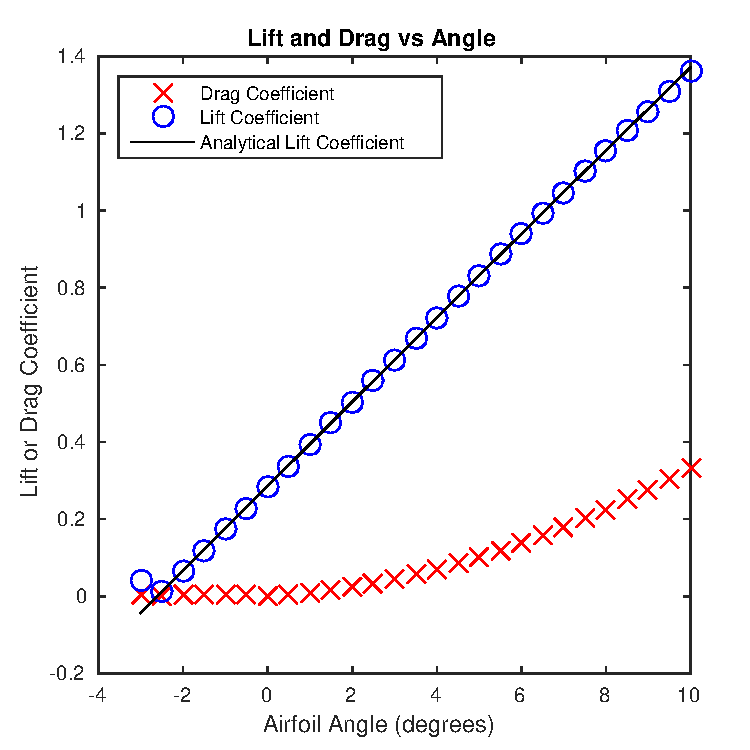
\includegraphics[scale=1.0]{LiftAndDrag.pdf}
\caption{The lift and drag coefficients as a function of angle of attack. The numerics closely match analytical results except the very first data point.}
\label{fig:liftanddrag}
\end{figure}

\begin{figure}
\centering
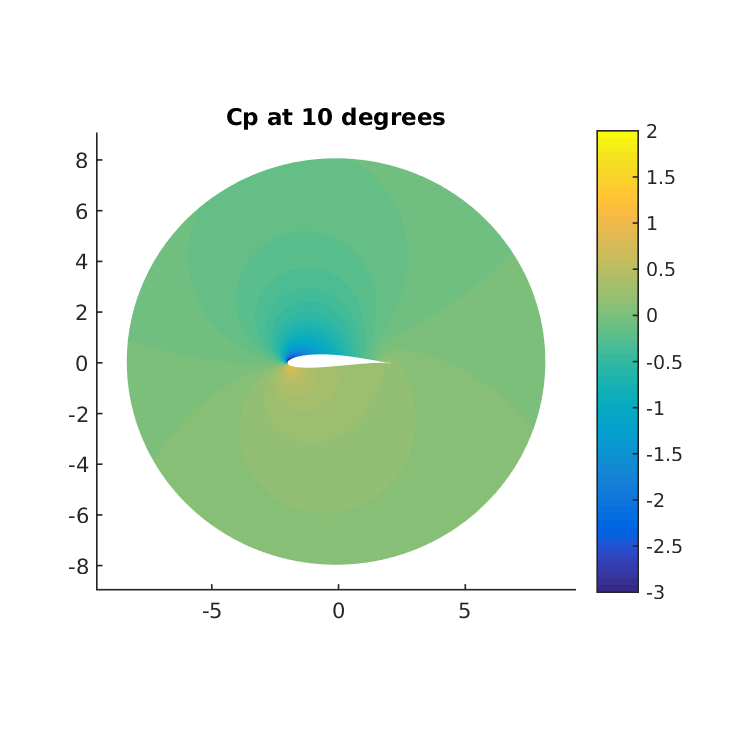
\includegraphics[scale=1.0]{Cp.png}
\caption{The scalar plot of the pressure coefficient. The range was truncated due to the singularity at the trailing edge.} 
\label{fig:Cp}
\end{figure}

\end{document}
